\section{Proposed Method}

MOEA/D-RAD, MOEA/D with on-line Resource Allocation by Diversity Metric, is the variant of MOEA/D proposed in this work. This algorithm uses the maximum relative diversity loss, MRDL, for determining the values of the utility function. 

\begin{algorithm}[h]
	\caption{MOEA/D-RAD}\label{alg1}
	\begin{algorithmic}[1]

	\State Initialize the weight vectors $\lambda_i$, the neighborhood $B_i$, the utility value $u_i$ every subproblem $i=1,...,N$.
		
		\While{\textit{Termination criteria}}
		\For {1 to N}
			\If{$\textit{rand()} < u_i$}\Comment{From MOEA/D-GRA}
				\State Generate a offspring $y$ for subproblem $i$.
				\State Update the population by $y$.
			\EndIf
	\EndFor
	\State Update \textit{\textbf{u}} by a diversity metric after $\Delta T$ generations.
		\EndWhile
	\end{algorithmic}
\end{algorithm}


The algorithm~\ref{alg1} describe MOEA/D-RAD. Except from line 4, in which a subproblem may not be part of the group that is going to be iterated and from line 7, in which the utility function is calculated, the whole procedure is similar to the MOEA/D-DE~\cite{zhang2009performance}. Likewise, all reproduction procedures and parameters are the same as in MOEA/D-DE~\cite{li2009multiobjective}. It is important to highlight that the neighborhood is only calculated in the initialization period.

%The update procedure is described The algorithm~\ref{alg2}, as in MOEA/D-GRA~\cite{zhou2016all}.
The decomposition method used is the Simple-Lattice Design (SLD), the scalar aggregation function Weighted Sum (WS), the Restricted update strategy.

We initialize the value of the vector $u=1$, as in MOEA/D-DRA. As in MOEA/D-DRA and GRA we have a learning period, $\Delta T$ generations (\textit{old function value}). Here, the $\Delta T=20$.   A sensitivity analyzes need to be performed for deciding suitable initial values for $u$ for $\Delta T$.

\subsection{Utility Function by Diversity} 

%\begin{figure}[!t]
%	\centering
%	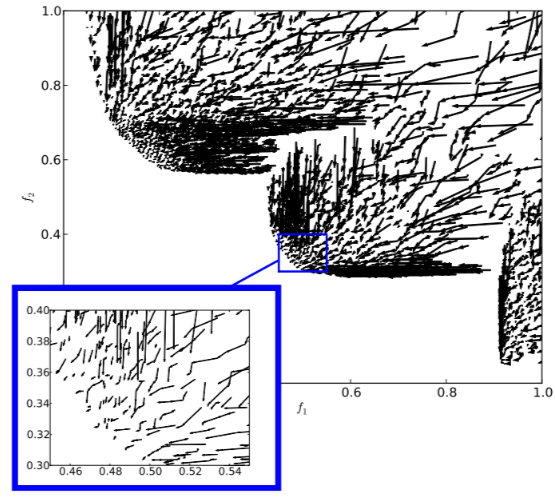
\includegraphics[width=0.47\textwidth]{img/conv_dir}
%	\caption{Estimated convergence directions over 500 generations in CEC-09 UF1 benchmark test problem.Figure from~\cite{gee2015online}}
%	\label{fig4}
%\end{figure}

The utility function proposed in this work is based on the Maximum Relative Diversity Loss MRDL. Prior to scalarizing it between $0$ and $1$ to fit the algorithm~\ref{alg1} we calculate MRDL for every individual of the population. The following function describes how to calculate the utility function given the MRDL, $\Gamma^{p \rightarrow c}$, as follows.

\begin{equation}
u_i = \Gamma^{p \rightarrow c}_i -  \Gamma^{p \rightarrow c}_j, \text{with  $i=1,...,N$.}
\end{equation}

%For the purpose of defining the utility function used in this work, we need to define the MRDL.

MRDL is an online diversity metric that estimates the diversity loss of a solution to the whole population~\cite{gee2015online}. First, it is an useful metric since if a new offspring generated is identical to any offspring solution in the convergence archive, the metric value will be infinite. Second, high values of  indicates the existence of similar offspring solution in the convergence archive or the offspring solution is close to the line of estimated convergence direction. Finally, it may be used as an adaptive technique to adjust parameters, as applied in its original study~\cite{gee2015online}.

The idea of the MRDL is to use the space movement (convergence directions) of a solution on the objective space towards the PF. The further an objective vector of a solution is from the convergence direction, more it contributes for the diversity of the approximated PF.

%This is done since the convergence direction is perpendicular to the diverse direction. Here we use the definition of convergence as solutions approaching to the POF in the objective space for the first, while for diversity as the spreading and distribution of solutions along the PF~\cite{gee2015online}.

To compute the MRDL, we need to estimate $k$ convergence directions at every generation. Then we need to  approximate the Relative Diversity Loss (RDL) for each of these $k$ convergence directions. To calculate this estimative of diversity loss of a solution to the whole population, the following equation is used, considering every incumbent solution related to a subproblem $i$, from the whole population.
 

\begin{equation}
\Gamma_{i}^{p \rightarrow c} = \underset{i=1,...,k}{\max} \Gamma_{d.conv_{y}}^{p \rightarrow c},
\end{equation}




RDL is a diversity measurement quantity that indicates the amount of diversity loss of an individual solution between two consecutive generations. High values of RDL imply a reduction of the solution spread and this equation may indicated the amount of diversity loss.

This quantity is given by a division between the shortest distance of a parent, $p$,  and offspring, $c$, to the line of convergence direction.

\begin{equation}
\label{rdl}
\Gamma_{d.conv_{y}}^{p \rightarrow c} = \dfrac{ ||p \prime - proj_{d.conv_{y}}p \prime|| }{||c \prime - proj_{d.conv_{y}}c \prime||}
\end{equation}

The numerator in~\ref{rdl} is the closest distance between the parent solution ($p$) to the convergence direction $(c_r - p_r)$. While, the denominator in~\ref{rdl} is the closest distance between the offspring solution ($c$) to the convergence direction $(c_r - p_r)$. %The projections of $p\prime$ and $c\prime$ objective vectors onto the convergence direction $d.conv_{y}$ are $proj_{d.conv_{y}}p \prime$ and $proj_{d.conv_{y}}c \prime$.

with $p\prime$ and $c\prime $ given by:

\begin{equation}
\begin{split}
p\prime = p - p_r,\\
c\prime = c - c_s,\\
\end{split}
\end{equation}
%verify this

with $p_r$ and $c_s$ being the parent and offspring objective vectors used to calculate the convergence direction in equation~\ref{1}. That is the index $s$ is equal to the index $j$ used to calculate $conv_{y}$. The same principle is valid for the index $r$.
 
The vector projection between two vectors is defined as next.

\begin{equation}
proj_{d.conv_{y}}p \prime = \frac {{d.conv_{y}} \cdot {p \prime}} {|{p \prime}|^2}{{p \prime}}.
\end{equation}

While the norm of $p \prime - proj_{d.conv_{y}}p \prime$ is calculated as follows.


\begin{equation}
||p \prime - proj_{d.conv_{y}}p \prime|| = sqrt(crossprod(proj_{d.conv_{y}}p \prime))
\end{equation}

and the norm of $c \prime - proj_{d.conv_{y}}c \prime$ is calculated similarly.


To estimate the convergence direction, $d.conv_{y}$, we need to have a offspring, $c_j$, that dominates a parent. Select a parent, $p_h$, solution that is closest to this offspring in the objective space. 

For every weakly dominated parent, one convergence direction is calculated as in the next equation.
\begin{equation}
\label{1}
	d.conv_{y} = c_j - p_h
\end{equation}

The index $j$ (for indexing offsprings, $c_j$) is selected from the set $D_c$. The index $h$ is explained later.

\begin{equation}
\label{D}
	D_c = \{d| \exists c_d \prec p_k, k \in {1,..., N}, d \in [1,..., |C|]\}
z\end{equation}

$N$ is the parent population size, $|C|$ is the size of the offspring population $C$. In equation~\ref{D}, the offspring $c_d$ must weakly dominate at least one parent solution. 

As from Zitzler et al.~\cite{zitzler2003performance} study, weak dominance ($A \succeq B$) means that any solution in B is weakly dominated by a solution in A. However, this does not rule out equality, because $A \succeq A$ for all approximation sets $A \in \Omega$.

The index $h$ (for indexing parents, $p_h$) comes from the following two equations.
\begin{equation}
h = \underset{k \in D_p }{argmin} || p_k - c_j ||
\end{equation}

\begin{equation}
\label{D_p}
D_p = \{k| \exists c_j \prec p_k, k \in {1,..., N}\}
\end{equation}

$D_p$ in equation~\ref{D_p} denotes the index set of parent solutions which are weakly dominated by $c_j$ (the $j$ index comes from equation~\ref{D}).


%\paragraph{Estimating diversity direction given the convergence direction} Diversity direction is define in~\cite{gee2015online} as the direction which is perpendicular to the converge direction.








